\documentclass[10pt,a4paper]{article}
\usepackage[utf8]{inputenc}
\usepackage{amsmath}
\usepackage{amsfonts}
\usepackage{amssymb}
\usepackage{float}
\newcommand\tab[1][1cm]{\hspace*{#1}}
\newcommand{\head}[1]{\textnormal{\textbf{#1}}}
\usepackage{graphicx}
\usepackage{scrextend}
\usepackage{wrapfig}
\usepackage{enumitem}
\author{Konrad Cybulski}
\title{Investigating the Effect of Different Data Normalization Techniques on Time Series Classification Accuracy}
\begin{document}
\begin{titlepage}
    \begin{center}
        \vspace*{1cm}
        
        \LARGE
        \textbf{Investigating the Effect of Different Data Normalization Techniques on Time Series Classification Accuracy}
        
        \vspace{4cm}
        
		\Large 
        
        \textbf{Konrad Cybulski}
        
        
        \LARGE
        \vspace{2cm}

        
        
        \vfill
        
        
        
        Research Proposal \\
        FIT2082 Research Project
        
        
        
\includegraphics[width=0.4\textwidth]{Images/monash_emblem.jpg}
              
        
        \large
        Faculty of Information Technology\\
        Monash University\\
        Australia\\
        15/08/2017
        
    \end{center}
\end{titlepage}

\pagebreak
\tableofcontents
\pagebreak

\section{Introduction} 

The UCR Time Series Classification Archive [1] is a data repository with over 1200 downloads and hundreds of references. 
While the classification accuracy shown by predictive models on the UCR data is irrefutable, we aim to investigate the effect on classification accuracy the methods used in data normalization have had. 
With data normalization techniques known to have significant impacts on prediction accuracy on many classifiers, in order to verify the accuracy of classification models an understanding of the impact of techniques used by UCR is necessary.
\\\\
The UCR Time Series Classification Archive is used as a benchmark dataset for hundreds of time series classification publications.
As explored by Keogh \& Kasetty [3], there exists a real need for larger testing on real world data due to the bias introduced into time series classification techniques developed and tested on a single benchmark dataset.
We aim to determine however whether it is not only the data on which techniques may be over-trained, but the normalization involved in creating such datasets.
\\\\
The raw unprocessed and non-normalized UCR data has been collected from Anthony Bagnall and Eamonn Keogh with the help of Geoff Web.


\section{Background}

This background focuses on the techniques used in normalization, and literature in the area of the effect of normalization techniques on classifier (and regressor) accuracy.

\subsection{Effect of Normalization on Time Series Classification Accuracy}

Methods of normalization are known to greatly affect the accuracy of classification in multivariate data sets.
When there exists data from two distributions which have greatly different means and variances, normalization becomes an important factor in ensuring each variable does not skew prediction.
In univariate datasets this may be less important.
However despite this, in a number of predictive models, including neural networks and support vector classifiers, the multidimensional problem space becomes not only easier to train for, but additionally a number of mathematical functions depend on normalized data.
In neural networks, the chosen activation functions depend heavily on this fact, with sigmoid activations becoming almost meaningless unless input is within the 0-1 range.
Support vector machines require a standardised problem space if the hyperplanes used in the separation of classes can be fitted most accurately.
While this itself is a more complex problem, we will focus on time series length standardisation, which is a more pressing and time series related problem.
\\\\
The UCR Time Series Data Archive's [1] cleaned data has a fixed time series length in each data set, while each data set has a vastly different length, it is important to recognize the effect this has on classification.
One reason DTW distance measures are so effective is due to the different rates at which events occur across a number of occurrences.
When an event may be registered in given amount of time, the same event might occur in a larger time frame in another occurrence, which using euclidean distance measurements would not match.
This event cannot be solved by changing the time series length, however time series length is integral in determining how much information is required in a given time series to have optimal results.
If a very small time series length is required to achieve high classification accuracy, the remainder of the raw time series is not required.
This idea is similar to the notion of early detection, which is a separate area of time series classification.
By changing time series length, both where they begin, and when they end, we control what section of the information and how much of it we allow classifiers to use for prediction.
\\\\
While more information allows for greater predictive accuracy, it may also introduce noise to the data, and additionally, the larger the data, the longer classification takes. 
Changes in time series length allows us to understand the information gain/loss, and the slow-down/speed-up associated with it. 


\section{Methodology}

This methodology briefly states the platforms which have been used to investigate the raw UCR data as introduced above as well as the nature of the data that has been used in this research.

\subsection{Data}

The original UCR Time Series Classification Archive [1] data is not only normalized using z-score normalization, it is additionally split into both training and testing subsets of the full dataset. 
The raw data available for this project is the data that was used to derive the UCR datasets CricketX, CricketY, CricketZ, GesturesX, GesturesY, GesturesZ and Wafer.
However we define these datasets as Cricket, Gestures and Wafer, and each of the multidimensional datasets (Cricket \& Gestures) will be investigated as three separate datasets.
In testing the accuracy of classification on this data, we take two approaches.
The first involving random train/test splits of the same size for a given data set which will provide a distribution of classification accuracy allowing for further analysis of the effect of time series length or normalization techniques in classification.
The second method is used to determine if any differences exist between the raw data and the UCR repository data.
This involves the matching of each time series in the raw data with its closest matching time series in the UCR repository data to determine if any significant differences exist between the two datasets.

\subsection{Normalization Techniques}

\subsubsection{Scalar Normalization}

The original UCR Time Series Classification Archive [1] data is normalized using z-score normalization.
We aim to investigate the two most common scale normalization techniques: z-score normalization and \textit{min-max} normalization.
Z-score normalization is most common and is most representative of the original raw data when it conforms to a normal distribution.
Z-score normalization involves converting each data point into a positive or negative value representing how many standard deviations away from the mean the data point is.
\textit{Min-max} normalization involves converting data into values between 0 and 1 by subtracting the minimum and dividing by the difference between the minimum and maximum values of the time series.
These normalization techniques are simple and are very commonly used in order to remove the bias involved in variable with large values compared to other smaller valued data.

\subsubsection{Time Series Length Normalization}

The original UCR Time Series Classification Archive [1] data is structured such that each time series in a given dataset is of the same length.
In datasets such as Cricket, where the lengths of time series have a very small variance from the mean, there is little need for strict normalization procedures with regard to time series length.
Despite this, time series length minimisation offers a drastic computational speed-up with respect to nearest neighbour algorithm run times.
In this research we examine the effect of both increasing and decreasing length of time series'. 
Both methods involve shrinking/expanding a time series of length \textit{n} to a standard length \textit{m}. 
\\\\
For a time series \textit{T} of length \textit{n}, we denote the \textit{i}-th data point in \textit{T} as $\textit{T}_{i}$.
We convert \textit{T} to a time series of length \textit{m}, which we denote as \textit{S}.
\\\\
Thus we create the new time series \textit{S} where each data point in \textit{S} is as follows:
\begin{center}
$\textit{S}_{i} = \textit{T}_{j}$ \tab $j = \lfloor n \times \dfrac{i}{m} \rfloor$
\end{center}
This results in information loss when \textit{m} < \textit{n}, the impact of which will be investigated.


\subsection{Classification Techniques}

The UCR Time Series Classification Archive [1] specifies the lowest classification error possible using a number of techniques.\\
1-NN Euclidean - This is the error using a one nearest neighbour algorithm with a euclidean distance measure.\\
1-NN DTW Best Warping Window - The warping window is a hyper-parameter in the NN-DTW classification method which has been determined for each data set along with the error achieved with this optimal window.\\
1-NN DTW No Warping Window - This is the error when no warping window is used in the NN-DTW classifier.\\
With solely these three techniques we will determine the accuracy of normalized data.
We choose to use these three techniques alone due to their power in time series classification [2] and the generality and simplicity of the algorithms.
\\\\
While other methods exist and may provide more accurate classifications, the use of NN classifiers will allow a better understanding of the homogeneity and relatedness of the normalized data within a given class.

\pagebreak
\section{Results}

\begin{figure}[H]
\begin{center}
	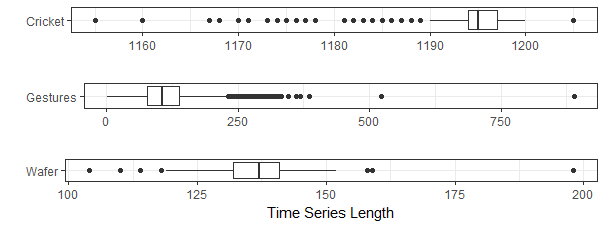
\includegraphics[width=1\textwidth]{Images/TimeSeriesLength_bydataset.png}
	\caption{The distribution of time series length for each of the three datasets investigated.}
\end{center}
\end{figure}

\subsection{Euclidean Distance Measure}

\begin{figure}[H]
\begin{center}
	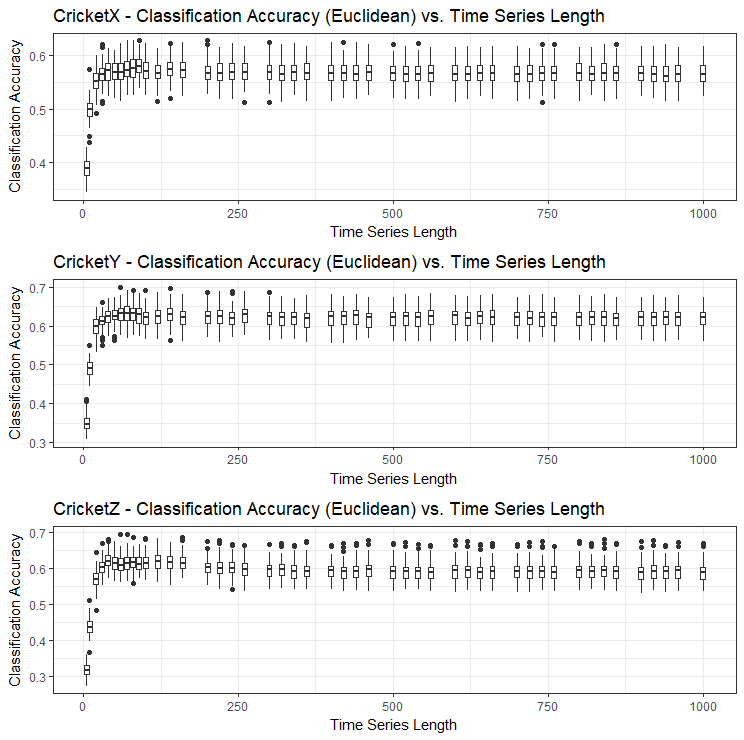
\includegraphics[width=1\textwidth]{Images/CricketAccuracyVsLengthEUCLIDEAN_box.png}
	\caption{The distribution of classification accuracy for the \textit{Cricket} dataset as a function of time series length using the Euclidean distance measure in NN prediction.}
\end{center}
\end{figure}

\begin{figure}[H]
\begin{center}
	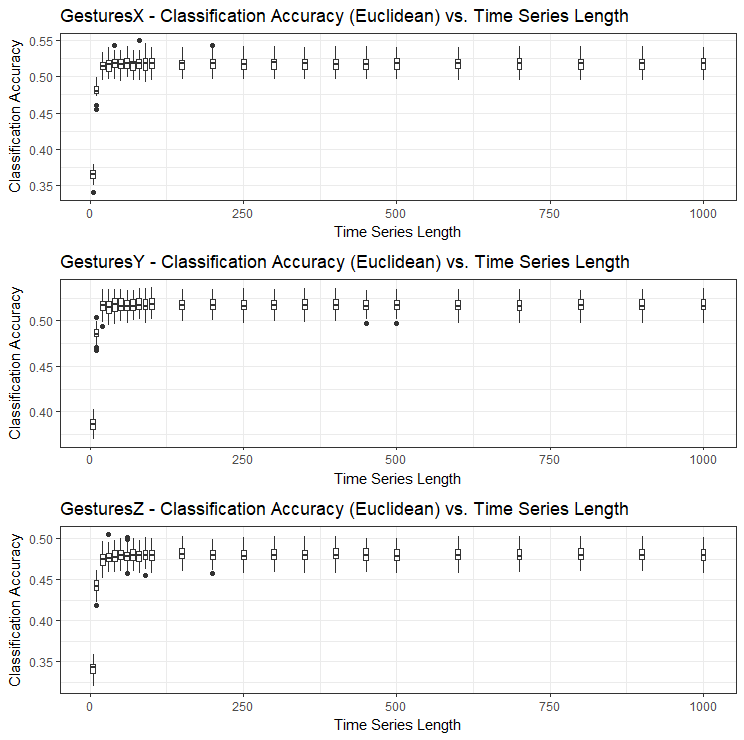
\includegraphics[width=1\textwidth]{Images/GesturesAccuracyVsLengthEUCLIDEAN_box.png}
	\caption{The distribution of classification accuracy for the \textit{Gestures} dataset as a function of time series length using the Euclidean distance measure in NN prediction.}
\end{center}
\end{figure}

\begin{figure}[H]
\begin{center}
	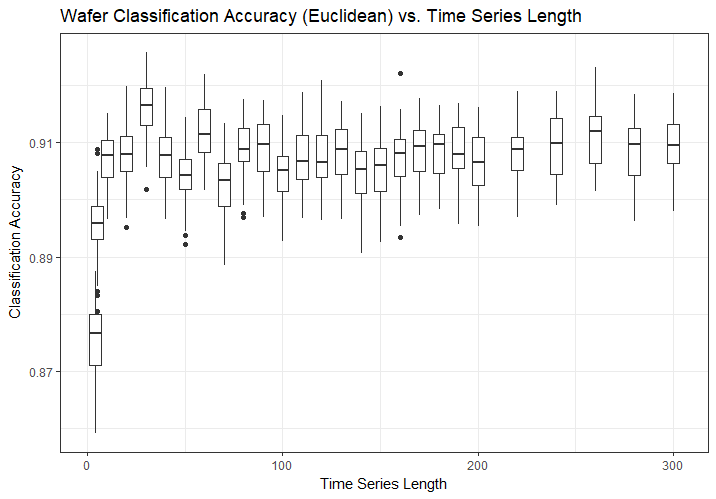
\includegraphics[width=1\textwidth]{Images/WaferAccuracyVsLengthEUCLIDEAN_box.png}
	\caption{The distribution of classification accuracy for the \textit{Wafer} dataset as a function of time series length using the Euclidean distance measure in NN prediction.}
\end{center}
\end{figure}

\subsection{DTW Distance Measure}

\begin{figure}[H]
\begin{center}
	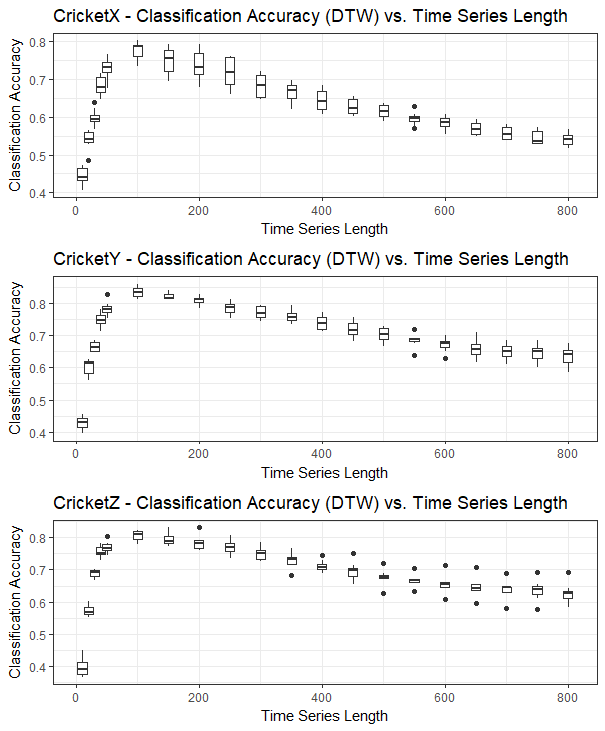
\includegraphics[width=1\textwidth]{Images/CricketAccuracyVsLengthDTW_box.png}
	\caption{The distribution of classification accuracy for the \textit{Cricket} dataset as a function of time series length using the DTW distance measure in NN prediction.}
\end{center}
\end{figure}

\begin{figure}[H]
\begin{center}
	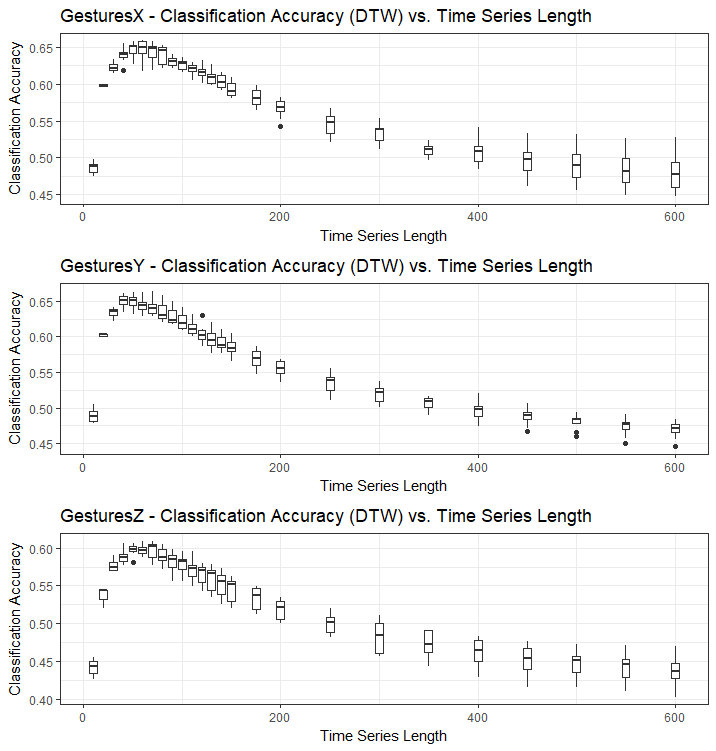
\includegraphics[width=1\textwidth]{Images/GesturesAccuracyVsLengthDTW_box.png}
	\caption{The distribution of classification accuracy for the \textit{Gestures} dataset as a function of time series length using the DTW distance measure in NN prediction.}
\end{center}
\end{figure}

\begin{figure}[H]
\begin{center}
	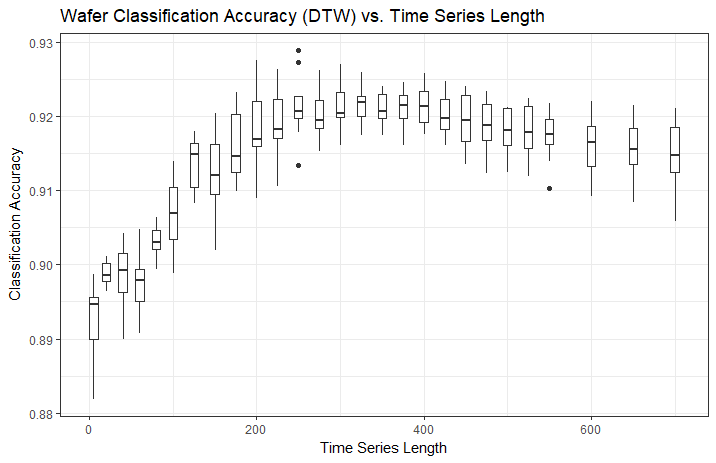
\includegraphics[width=1\textwidth]{Images/WaferAccuracyVsLengthDTW_box.png}
	\caption{The distribution of classification accuracy for the \textit{Wafer} dataset as a function of time series length using the DTW distance measure in NN prediction.}
\end{center}
\end{figure}


\section{Discussion}

\subsection{Scalar Normalization}



\subsection{Time Series Length Normalization}
This section of the report focuses on the effects of time series length normalization on each of the three datasets investigated.
\\\\
While each of the datasets are quite different in nature, we find clear similarities with regard to both Euclidean distance measures as well as DTW distance measures with respect to classification accuracy.

\subsubsection{Euclidean Distance Measure}
The data collected for all three datasets using a Euclidean distance measure for Nearest Neighbour Classification shows there exists an optimal time series length for Euclidean NN classification.
In \textit{Figure 2} \& \textit{Figure 3} we observe the classification accuracy approaches a maximum as the time series length increases.
However this maximum classification accuracy is reached at a very small time series length  and remains almost stable as the length continues to increase.
\\\\
Here we introduce the idea of a minimum time series representation (MTSR) which additionally minimise information loss in the data (maximise classification accuracy).
In the case of \textit{Cricket}, we have a minimum information loss at a time series length close to the initial values of the time series', ~1200.
However while this minimises the information loss, we are able to achieve the same classification accuracy at a time series length of 40, and a marginally higher distribution of classification accuracy for a time series length of 90.
The main benefit of a MTSR is faster classification due to the reduced computational complexity of performing Euclidean distance measurements on a smaller time series.
\\\\
In the \textit{Wafer} dataset, as shown in \textit{Figure 4}, we observe similar results, where the classification accuracy remains stable as the time series length increase.
In this dataset, we see a clear maximum classification accuracy for a length of 30.
However we obtain a similar accuracy distribution with a time series length of 10-20 as we do with a length of 300.


\subsubsection{DTW Distance Measure}
The classification accuracy results using a DTW distance measure differ significantly from the results and findings using Euclidean distance measures.
Each of the three datasets show a clear maximum classification accuracy.
With each of the datasets having an optimal time series length and classification accuracies as below:\\

\begin{tabular}{lcccc}
\hline
\head{Dataset} & \head{Avg. Accuracy} & \head{Optimal Length} & \head{Optimal Accuracy}\\
\hline
CricketX & 0.6299 & 100 & 0.7756 \\
CricketY & 0.7063 & 100 & 0.8353 \\
CricketZ & 0.6888 & 100 & 0.8061 \\
\hline
GesturesX & 0.5768 & 60 & 0.6459 \\
GesturesY & 0.5708 & 40 & 0.6498 \\
GesturesZ & 0.5293 & 50 & 0.5975 \\
\hline
Wafer & 0.9142 & 325 & 0.9214 \\
\hline

\end{tabular}
\\\\
In both \textit{Cricket} and \textit{Gesture} datasets there is a significant absolute increase in the classification accuracy.
While \textit{Wafer} appears to be only a marginal improvement in classification accuracy, in comparison to accuracy at different time series lengths, the accuracy is 0.77 standard deviations above the mean accuracy across all lengths shown.
This increase above the mean accuracy holds for both \textit{Cricket} and \textit{Gestures} as well, with optimal time series length accuracy in \textit{Cricket} being 1.66, 1.36 and 1.24 standard deviations above the mean for \textit{Cricket} X, Y and Z respectively.
\textit{Gestures}, with optimal time series length accuracy 1.12, 1.23 and 1.15 standard deviations above the mean for \textit{Gestures} X, Y and Z respectively.
\\\\
These are all significant improvements to the average accuracy for other time series lengths, however the most notable aspect of these results is that there exists an optimal time series length that maximises the accuracy when using DTW.
In contrast to Euclidean measures, where there exists a minimal representation of the time series that still maximises the classification accuracy, DTW has a clear maximum with respect to time series length.
Due to the single maximum, there also exists some symmetry, where on either side of the optimal length, there are lengths that result in the same accuracy.
For example, in \textit{Cricket}, time series lengths of 30 and 550 result in extremely similar classification accuracy, however in order to maximise speed of computation, choosing the length of 30 would be optimal.
\\\\

TALK ABOUT WHY THE OPTIMAL LENGTH IS THAT LENGTH, I>E> I DUNNO


\section{Conclusions}

Euclidean distance measures, while known to be a less accurate measure than DTW in time series classification, shows to be more stable than DTW.
DTW in comparison, shows to have an optimum time series length for maximum classification accuracy.

\section{Further Work}

Due to only three datasets being available to this research, our findings are localised to the datasets discussed.
While our conclusions regarding time series length and normalization techniques with respect to these datasets hold true, the nature of the data is important in relation to classification accuracy.
Due to this, more work is required to understand the effect of time series length normalization and scalar normalization on other data from both the UCR Time Series Classification Archive [1] and other data.
Additionally further investigation is required into multivariate time series. 
As discussed in this report, the information loss associated with the reduction of time series length impacts the classification accuracy (both positively and negatively).
More research is required to find more intricate models for finding minimum time series representations which minimise information loss.


\pagebreak
\begin{thebibliography}{9}

\bibitem{1}
Yanping Chen, Eamonn Keogh, Bing Hu, Nurjahan Begum, Anthony Bagnall, Abdullah
Mueen and Gustavo Batista (2015). The UCR Time Series Classification Archive. URL $www.cs.ucr.edu/~eamonn/time_series_data/$

\bibitem{2}
Petitjean, F., Forestier, G., Webb, G. I., Nicholson, A. E., Chen, Y., \& Keogh, E. (2016). Faster and more accurate classification of time series by exploiting a novel dynamic time warping averaging algorithm. \textit{Knowledge and Information Systems}, 47(1), 1-26.

\bibitem{3}
Keogh, E., \& Kasetty, S. (2003). On the need for time series data mining benchmarks: a survey and empirical demonstration. \textit{Data Mining and knowledge discovery}, 7(4), 349-371.

$www.cs.ucr.edu/~eamonn/time_series_data/$

\end{thebibliography}

\end{document}
